
\documentclass[10pt,compress,xcolor={usenames,dvipsnames}]{beamer} %slides and notes
\usepackage{amsmath,datetime,xmpmulti,mathtools,bbm,mathabx,array,booktabs,alltt,xspace,tikz,calc,colortbl,graphicx}
\usepackage[usenames]{xcolor}
\usepackage[tikz]{mdframed}
\usepackage[author-year]{amsrefs}
\usepackage{newpxtext}
\usepackage[euler-digits,euler-hat-accent]{eulervm}
\usetikzlibrary{arrows}
\usepackage{cleveref}
\usepackage{multicol}
\usepackage{caption}
\usepackage{subcaption}
\usepackage{algorithm}
\usepackage{algorithmicx}% http://ctan.org/pkg/algorithm
\usepackage{algpseudocode}% http://ctan.org/pkg/algorithmicx




%%%%%
% Using Freds theme
%%%%%%%%%
\usetheme{FJHSlimNoFoot}


%%%%%
% Definitions from Freds Latex
%%%%%%%%%

\definecolor{ltred}{rgb}{0.75,0.8,0.75}

\setlength{\parskip}{2ex}
\setlength{\arraycolsep}{0.5ex}

\makeatletter
\newcommand{\vast}{\bBigg@{3}}
%\newcommand{\vast}{\bBigg@{4}}
\newcommand{\Vast}{\bBigg@{5}}
\makeatother


\title[]{Fast automatic Bayesian Cubature \\
	with Lattice sampling
\\[1.0ex] }
\author[]{Jagadeeswaran R.}
\institute{Department of Applied Mathematics,  Illinois Institute of Technology, Chicago IL
\\
\href{mailto:jrathin1@iit.edu}{\url{jrathin1@iit.edu}} }
\thanksnote{
Thanks to my adviser Prof. Fred J. Hickernell\\[1.5ex]
Thanks for attending my presentation }
\date[]{ \textbullet\ Feb 27, 2019 \textbullet\ }

%% where the figures are stored
\graphicspath{{figures/}}
%\graphicspath{{./figures/}{/home/jagadees/MyWriteup/Sep_2ndweek/}}
%\graphicspath{{D:/Dropbox/writeup/BeamerPresent/}{D:/Dropbox/writeup/BeamerPresent/figures/}{D:/Mega/MyWriteupBackup/Sep_2ndweek/}}


\mdfdefinestyle{redshade}{%
	leftmargin=0 pt,
	rightmargin = 0pt,
	innerleftmargin = 1ex,
	innerrightmargin = 1ex,
	skipabove = 0 pt,
	skipbelow = 0 pt,
	backgroundcolor=red!20,
	linecolor=red!20,
	roundcorner=5pt}


\input FJHDef.tex
\newcommand{\bm}[1]{\boldsymbol{#1}}
\renewcommand{\mSigma}{\Sigma}
\renewcommand{\mLambda}{\Lambda}
\newcommand{\smallcite}[1]{{\small\cite{#1}}}
\newcommand{\smallocite}[1]{{\small\ocite{#1}}}
\newcommand{\smallcites}[1]{{\small\cites{#1}}}
\newcommand{\tol}{\text{tol}}
\newcommand{\Dt}{\text{D}}
\newcommand{\Ex}{\mathbb{E}}
\newcommand{\modop}[1]{{\left\lbrace{#1}\right\rbrace}}
\newcommand{\Ba}{\text{B}}
\newcommand{\hvtheta}{\hat{\vtheta}}

\newcommand{\MLE}{\textup{MLE}}
\newcommand{\GCV}{\textup{GCV}}
\newcommand{\full}{\textup{full}}
\newcommand{\vC}{\bvec{C}}
\newcommand{\vW}{\bvec{W}}

\newcommand{\tvv}{\tilde{\vv}}

\newcommand{\mCtheta}{\mC_{\vtheta}}
\newcommand{\mCInv}{\mC^{-1}}
\newcommand{\tmC}{\widetilde{\mC}}

\newcommand{\D}[1]{\text{d}{#1}}
\newcommand{\dvx}{\dif {\vx}}
\newcommand{\dvt}{\dif {\vt}}
\newcommand{\vthetaMLE}{{\vtheta}_{\MLE}}
\newcommand{\vrho}{\bm{\rho}}

\newcommand{\err}{{\text{err}}}
\newcommand{\errn}{{\text{err}}_{\text{n}}}
% \newcommand{\errtol}{{\text{err}}_{\text{tol}}}
% \newcommand{\errtol}{\text{tol}}
\newcommand{\errtol}{{\epsilon}}
\newcommand{\abstol}{{\text{err}}_{\text{abs}}}
\newcommand{\reltol}{{\text{err}}_{\text{rel}}}

\newcommand{\tmLambda}{\widetilde{\mLambda}}

\newcommand{\tB}{\widetilde{B}}
\newcommand{\tvC}{\widetilde{\vC}}

\newcommand{\financePict}
{\href{http://i2.cdn.turner.com/money/dam/assets/130611131918-chicago-board-options-exchange-1024x576.jpg}
 {\includegraphics[height =
1.7cm]{130611131918-chicago-board-options-exchange-1024x576.jpg}}}

\newcommand{\GaussPict}
{\href{http://www.mathworks.com/matlabcentral/answers/uploaded_files/26298/Plotting\%20a\%203d\%20gaussian\%20function\%20using\%20surf\%20-\%202015\%2002\%2027.png}
 {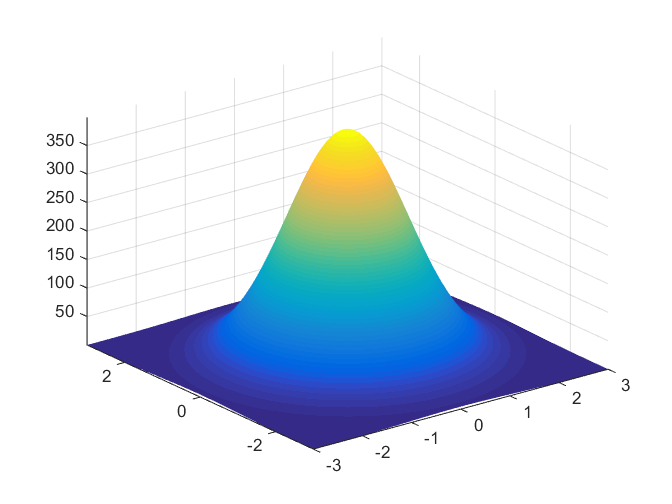
\includegraphics[height
 = 2cm]{Plotting_gaussian.png}}}

\DeclareMathOperator{\Var}{VAR}
\DeclareMathOperator{\disc}{DSC}
\DeclareMathOperator{\algn}{ALN}
%\DeclareMathOperator{\GP}{\cg\cp}

\newcommand{\redroundmathbox}[1]{\parbox{\widthof{$#1$\hspace{1em}}}
	{\begin{mdframed}[style=redshade]\centering $#1$ \end{mdframed}}}
\newcommand{\setbeameruncoveredtransp}{\setbeamercovered{transparent=10}}

\def\abs#1{\ensuremath{\left \lvert #1 \right \rvert}}


\makeatletter
\patchcmd{\beamer@sectionintoc}
  %{\vfill}
  {\vskip\itemsep}
  %{}
  %{}
\makeatother

\algdef{SE}[DOWHILE]{Do}{doWhile}{\algorithmicdo}[1]{\algorithmicwhile\ #1}%



\begin{document}
\tikzstyle{every picture}+=[remember picture]
\everymath{\displaystyle}


\frame{\titlepage}







\iffalse

%\frame{\frametitle{Table of contents}\tableofcontents}
\begin{frame}{\contentsname}
    \begin{minipage}{\textwidth}
    	\vspace{-6ex}
		\linespread{1.4}
		\begin{multicols}{2}
		\tableofcontents
		\end{multicols}
    \end{minipage}
\end{frame}
\fi

\section{Introduction}
\frame
{
\frametitle{Numerical Integration}
\vspace{-5ex}
A fundamental problem in various fields, including finance, machine learning and statistics.
\vspace{-2ex}
\begin{align*}
\mu = \int_{\reals^d} g(\vx) \,  \dif \vx = \int_{[0,1]^d} f(\vx) \,
\dif\vx  = & \Ex[f(\vX)], \quad \text{where} \quad \vX \sim \cu [0,1]^d
\end{align*}
\vspace{-5ex}
\begin{align*}
\text{by a  cubature rule} \quad
\hmu_n := & w_0 + \sum_{j=1}^{n} f(\vx_j) w_j \qquad
\\
\qquad \text{using  points $\{\vx_j \}_{j=1}^{n}$ and associated weights $w_j$.}
\end{align*}
\pause
%\vspace{-3ex}
%using  points $\{\vx_j \}_{j=1}^{n}$ and associated weights $w_j$.
The goal of this work is to
\vspace{-3ex}
\begin{itemize}
\item Develop an automatic algorithm for integration
\item Assume \alert{$f$} is drawn from a Gaussian process
\begin{itemize}
\item Need to estimate the mean and Covariance kernel
\end{itemize}
\item MLE is expensive in general
\begin{itemize}
\item Use points and kernel for which MLE is cheap
\end{itemize}
\item Use an \alert{extensible} point-set and an algorithm that allows to add more points if needed
\item Determine \alert{$n$} such that, given \alert{$\errtol$}, $\abs{\mu-\hmu_n} \leq \errtol$
\end{itemize}
}







\begin{frame}[label = Problem]
\frametitle{Motivating Examples }
\vspace{-5ex}
\begin{tabular}{m{8.5cm}m{2.7cm}}
\vspace{-1ex}
\[
\text{Gaussian probability} =
\int_{[\va, \vb]}
\frac{\me^{-\vx^T\mSigma^{-1}\vx/2}}{(2\pi)^{d/2}\abs{\mSigma}^{1/2}}\,\dif\vx
, \; \text{\smallcite{Gen93}}
\]  & \GaussPict
\tabularnewline [-1.2ex] \arrayrulecolor{ltred} \toprule
\tabularnewline [-1ex]
\uncover<2->{
\vspace{-3ex}
\begin{gather*}
\text{Option pricing} =
\int_{\reals^d}
{
\text{payoff}(\vx)} \,
\underbrace{
\frac{\me^{-\vx^T\mSigma^{-1}\vx/2}}{(2\pi)^{d/2} \abs{\mSigma}^{1/2}}}_{\text{PDF of Brownian motion at $d$ times}}\,\dif\vx, \; \text{\smallcite{Gla03}}
\\
\text{where} \quad \text{payoff}(\vx) =  \me^{-rT}
\max\left(\frac 1d \sum_{k=1}^d S_k(x_k) - K, 0 \right)
\\
S_j(x_j) = S_0 \me^{(r -\sigma^2/2)t_j +
\sigma x_j} =\text{stock price at time } t_j = jT/d; 
\end{gather*}
\vspace{-1ex}
}
\tabularnewline [-1.2ex] \arrayrulecolor{ltred} \toprule
\tabularnewline [-1ex]
\uncover<3->{
\vspace{-3ex}
\begin{gather*}
\text{Keister integral}  = \int_{\mathbb{R}^d} \cos(\lVert \vx \rVert)
\exp(-\lVert \vx \rVert^2) \,  \dvx, \quad
 d = 1, 2, \ldots \; \text{\smallcite{Kei96}}
\end{gather*}
}
\end{tabular}
\end{frame}

































\subsection{Automatic cubature algorithm}

\frame{
\setbeameruncoveredtransp
%\frametitle{Algorithm }
\vspace*{-6ex}
\uncover<1-2>{
\begin{algorithm}[H]
  \begin{algorithmic}[1]
  \Procedure{AutoCubature}{$f$,$\errtol$} 
    %\Comment{Integrate within the error tolerance \alert{$\errtol$}}
	  \Require a generator for the sequence
	    $\vx_1, \vx_2, \ldots$; 
	    a black-box function, $f$; 
	    an absolute error tolerance,
	    $\varepsilon>0$; the positive initial sample size, $n_0$;
	    the maximum sample size $n_{\textup{max}}$
      % \State $n_0 \gets 2^8$ \Comment{start with minimum number of points}
      \State $n\gets n_0, \; n' \gets 0, \; \errn \gets \infty$
      %\Do
      \While{$\errn > \varepsilon$ and $n \le n_{\textup{max}}$} %\Comment{Iterate till error tolerance is met}
        \State Generate $\{ \vx_i\}_{i=n' + 1}^{n}$ and sample $\{f(x_i)\}_{i=n'+1}^{n}$, 
        \State Compute $\vtheta$
        \State Compute error bound \alert{$\errn$ } %\Comment{$\errn$ data driven error bound}
        %\If{\alert{$\errn \leq \errtol$}}
	    %    \textbf{break}
        %\EndIf
        \State $n' \gets n, n\gets 2 \times n'$
      \EndWhile
      \State Sample size to compute $\hmu$, $n \gets n'$
      % \State Compute cubature weights $\{ w_i \}_{i=1}^{n}$
      \State Compute approximate $\hmu_n$, the approximate integral
      \State \textbf{return} $\hmu_n$ \Comment{Integral estimate $\hmu_n$}
  \EndProcedure
  \end{algorithmic}
  %\caption{Template}\label{algorithmBasic}
\end{algorithm}}
\vspace*{-4ex}
\uncover<2>{
\textbf{Problem:}
\vspace*{-4ex}
\begin{itemize}
\item How to choose \alert{$\{\vx_i\}_{i=1}^n$}, and
\alert{$\{w_i\}_{i=1}^n$} to make $\abs{\mu - \hmu_n}$ small? what is $\errn$? \alert{(Bayesian posterior error)}
\item How to find $n$ such that $\abs{\mu - \hmu_n} \le \errn \le \errtol $ ? \alert{(automatic cubature)}
\end{itemize}
}
}







\section{Bayesian cubature}


\subsection{Posterior Error}


\begin{frame}
\frametitle{Bayesian posterior error}
\vspace*{-4ex}
\alert{Assume random}
$f \sim \mathcal{GP} (m, s^2C_{\vtheta})$,
a \alert{Gaussian process} with mean $m$ and covariance kernel, $s^2C_{\vtheta}$, $C_{\vtheta}:[0,1] \times [0,1] \to \reals$ .
\vspace*{-1ex}
\begin{align*}
\text{Lets define} \; c_0 &= \int_{[0,1] \times [0,1]} C_{\vtheta} (\vx,\vt) \dvx \dvt, 
\\
\vc& = \left( \int_{[0,1] } C_{\vtheta} (\vx_i,\vt) \dvt \right)_{i=1}^n,
\quad
\mC =  \biggl( C_{\vtheta} (\vx_i,\vx_j) \biggr)_{i,j=1}^n
\end{align*}
\pause
\vspace*{-3ex}
\begin{align*}
\mu - \hmu_n  \big \vert \vy & \; \sim \;
\cn
\biggl(-w_0 +
m(1- \bm{1}^T \mathsf{C}^{-1}\vc) +
\vy^T (\mathsf{C}^{-1}\vc - \vw), \quad s^2(c_0 - \vc ^T \mathsf{C}^{-1} \vc)
\biggr)
\\
\text{where} \; \vy &= \bigl(f(\vx_i)\bigr)_{i=1}^n. \quad \text{Moreover \alert{$m, s$ and $\vtheta$} needs to be inferred}.
\\
\hmu_n &= w_0 + \sum_{i=1}^n w_i f(\vx_i) = w_0 + \vw^T \vy
\end{align*}
\pause
\vspace*{-3ex}
\begin{align*}
\text{In general choosing} \quad
w_0 & = m(1 - \vone^T \mCInv \vc)
, 
\;
\vw = \mathsf{C}^{-1}\vc, \; \text{ makes error unbiased }
\\
\text{If $\alert{m = 0}$ fixed, choosing} \quad
\vw & =
\mathsf{C}^{-1}\vc, \; \text{ makes error unbiased }
\end{align*}
\ocite{Dia88a}, \ocite{OHa91a}, \ocite{Rit00a}, \ocite{RasGha03a} and others
%\[ \mathbb{P}[\lvert\mu - \hat{\mu}_n\rvert \le \text{err}_n] =& 99\% \quad \text{for} \quad
%\text{err}_n = 2.58\sqrt{\bigl (c_{0} - \vc^T  \mC^{-1} \vc \bigr) \, s^2 }
%& \text{and $\mC^{-1}$ typically takes $\alert{\Order(n^3)}$ operations} \]
\end{frame}









\subsection{MLE}


\begin{frame}
\frametitle{Parameter estimation - Maximum likelihood}
\vspace*{-6ex}
The log-likelihood of the parameters given the data $\vy = (f(\vx_i))_{i=1}^{n}$ is :
\vspace*{-2.0ex}
\begin{align*}
\displaystyle
l(s,\vtheta|y)=
\log
\left[
\frac{1}
{\sqrt{(2\pi)^n\text{det}(s^2\mC)}}
\exp{\left(
-\frac{1}{2}s^{-2}{(\vy-m\bm{1})}^T \mC^{-1} (\vy-m\bm{1})
\right)}
\right]
%; \; \mC =  \left( C_{\vtheta} (\vx_i,\vx_j) \right)_{i,j=1}^n
\end{align*}
\pause
\vspace{-4ex}
\begin{align*}
\text{Maximising w.r.t }&\;  m \text{ and then $s^2$, further with $\vtheta$}: \;
\\
m_{\MLE} &= \frac{\bm{1}^T \mC^{-1} \vy}{\bm{1}^T \mC^{-1} \bm{1}}, \quad
s^2_{\MLE} =
\frac{1}{n} (\vy-m_{\MLE}\bm{1})^T \mC^{-1} (\vy-m_{\MLE}\bm{1})  , & \text{(Explicit)}
\\
\vthetaMLE &= \argmin_{\vtheta}
\log
\left(
\frac{1}{2n} \log(\det \mC) + \log(s_\MLE)
\right)
 & \text{(numeric)}
\\
\hmu_\MLE  &= 
\left(
\frac{ (1 - \vone^T  \mCInv\vc )  \vone }{ \vone^T \mCInv \vone}   +  \vc 
\right)^T  \mCInv \vy  , & \text{(Explicit)}
\end{align*}
\pause %\vspace{-3ex}
\alert{Why do we need $\vtheta_{\MLE}$?} \quad Function space spanned by $C_{\vtheta}$ customized to contain the integrand function $f$.
\end{frame}





\begin{frame}
\frametitle{Parameter estimation - Full Bayes}
\vspace*{-6ex}
Treat $m$ and $s$ as hyper-parameters with a non-informative, conjugate prior, namely $\vrho_{m,s^2}(\xi, \lambda) \propto 1/\lambda$.
Then the posterior density for the integral $\mu$ given the data is :
\vspace*{-2.0ex}
\begin{align*}
\rho_{\mu}(z | \vf = \vy)
& \propto \int_{0}^\infty \int_{-\infty}^\infty \rho_{\mu}(z | \vf = \vy, m = \xi, s^2 = \lambda)  
\rho_{\vf}(\vy | \xi, \lambda ) \rho_{m, s^2}(\xi, \lambda) \, \D \xi \D \lambda 
\\ & \propto \left(1 +  \frac{1}{n-1} \frac{(z - \mu_{\full})^2}{\widehat{\sigma}_{\full}^2} \right)^{-n/2}
\end{align*}
\pause
\vspace{-4ex}
\begin{align*}
\text{Where}: \;
\\
\mu_{\full} &= \mu_\MLE
\\
\hsigma^2_{\full} 
& = \frac{1}{n-1}
\vy^T\left[ \mC^{-1} 
- \frac{ \mC^{-1} \vone\vone^T \mC^{-1}}{\vone^T \mC^{-1} \vone}  \right]\vy
\times  \left[\frac{(1 - \vc^T \mC^{-1} \vone)^2}{\vone^T \mC^{-1} \vone} + (c_0  -\vc ^T \mC^{-1} \vc) \right]
\\ &\mathbb{P}_f \left[ |\mu-\hmu_{\full}|  \leq \err_{\full} \right]  = 99\%,
\\ \err_{\full} &:= t_{n_j-1,0.995} \hat{\sigma}_{\full} > \err_{\MLE}
\end{align*}
\end{frame}




\begin{frame}
\frametitle{Parameter estimation - Leave-one-out Cross validation}
\vspace*{-6ex}
Let $\widetilde{y}_i = \Ex[f(\vx_i ) | \vf_{-i} = \vy_{-i}]$.
The cross-validation criterion, which is to be minimized, is sum of squares of the difference between these conditional expectations and the observed values: :
\vspace*{-2.0ex}
\begin{align*}
\textup{CV} &= \sum_{i=1}^n (y_i - \widetilde{y}_i)^2 = \sum_{i=1}^n \left(\frac{\zeta_i }{a_{ii}} \right)^2, \quad \text{where}\; \bm{\zeta} = \mC^{-1}(\vy - m \vone), 
\\
& \qquad \qquad a_{ii} \; \text{are diagonal elems of} \; \mC^{-1} = \begin{pmatrix} a_{ii}  & \vA_{-i,i}^T \\  \vA_{-i,i} & \mA_{-i,-i}\end{pmatrix}
\\
\GCV &
= \frac{\sum_{i=1}^n\zeta_i^2}{\left(\frac 1n \sum_{i=1}^n a_{ii} \right)^2} 
= \frac{(\vy - m\vone)^T \mC^{-2} (\vy - m \vone)}{\left(\frac 1n \trace(\mC^{-1}) \right)^2}.
\end{align*}
\pause
\vspace{-4ex}
\begin{align*}
\vtheta_{\GCV} &= \argmin_{\vtheta} \left\{\log \left(  \vy^T \left[\mC^{-2} - \frac{\mC^{-2} \vone \vone^T \mC^{-2}}{\vone^T \mC^{-2} \vone}  \right] \vy \right)  
- 2 \log \left ( \trace(\mC^{-1}) \right ) \right\}
\\
s^2_{\GCV} & : = \vy^T \left[\mC^{-2} - \frac{\mC^{-2} \vone \vone^T \mC^{-2}}{\vone^T \mC^{-2} \vone}  \right] \vy  \left[ \trace(\mC^{-1}) \right]^{-1}, 
\quad m_{\GCV} := \frac{\vone^T \mC^{-2} \vy}{\vone^T \mC^{-2} \vone}. 
\end{align*}
\end{frame}





\iffalse

\subsection{Bayesian cubature : Summary}


\frame{
\frametitle{Bayesian cubature using MLE results : Summary}
\vspace{-8ex}
\begin{align*}
\text{Assume}  \; f &\sim \mathcal{GP} (m, s^2 C_{\vtheta}) \; \text{given} \;
\vy =\bigl( f(\vx_i) \bigr)_{i=1}^{n},
\\
\mu - \hmu_n & \big \vert \vy
\; \sim \;
\cn
\bigl(w_0 +
m(1- \bm{1}^T \mathsf{C}^{-1}\vc) +
\vy^T (\mathsf{C}^{-1}\vc - \vw), \quad s^2(c_0 - \vc ^T \mathsf{C}^{-1} \vc)
\bigr)
\end{align*}
\pause
\vspace{-4ex}
\begin{align*}
\;  m_\MLE = \frac{\bm{1}^T \mC^{-1} \vy}{\bm{1}^T \mC^{-1} \bm{1}},& \; \text{and} \; \quad
s^2_\MLE = \frac {1}{n} \vy^T
\left[ \mCInv - \frac{\mCInv \vone \vone^T \mCInv}{\vone^T \mCInv \vone}\right] \vy,
\\
\vthetaMLE &= \argmin_{\vtheta}
\log
\left[
\frac{1}{2n} \log(\det \mC) + \log(s_\MLE)
\right]
\\
 \;
\hmu_n &=  w_0 +  \vw^T \vy =
m_\MLE
(1 - \bm{1}^T \mC^{-1} \vc)
+ \vc^T\mathsf{C}^{-1} \vy,
\\
\mathbb{P}[\lvert\mu - \hat{\mu}_n\rvert \le \text{err}_n] & \geq  99\% ,
\\
\text{If} \quad
\text{err}_n & \leq 2.58 \; s_\MLE \; \sqrt{\bigl (c_{0} - \vc^T  \mC^{-1} \vc \bigr)}
\\
& \text{Where $c_0$, $\vc$ and $\mC$ depend on $\vthetaMLE$}
\end{align*}
\pause
\alert{Problem :} 
\\
$\mathsf{C}^{-1}$ typically requires \alert{$\Order(n^3)$} operations, which makes it impractical for large $n$.
}
\fi

























\iffalse

\frame{
\frametitle{Bayesian Cubature - Deterministic Interpretation}
\vspace{-7.8ex}
\begin{align*}
f \in & \cf \text{ with reproducing kernel } C_{\vtheta}
\\
\text{if }  &
\Var^{\Dt}(f - \tf_{\vy}) \le \frac{2.58}{\alert{\sqrt{n}}} \Var^{\Dt}(\tf_{\vy})
\end{align*}
\pause
\begin{align*}
\text{\alert{replace} } & C_{\vtheta} \text{ by } C_{\vtheta}
\\
\text{err}_n &= 2.58 \disc^{\Ba}(\nu - \hnu) \Var^{\Ba}(f)
\\
\vthetaMLE &= \argmin_{\vtheta}  \vol \bigl(\bigl( \vz \in \reals^n :
\quad \Var^{\Dt}_{\vtheta}(\tf_{\vz}) \le \Var^{\Dt}_{\vtheta}(\tf_{\vy}) \bigr) \bigr ) \\
\tf_{\vy}: & \; \text{minimum norm interpolant}
\end{align*}


}
\fi






\iffalse
\begin{frame}<1>[label=BayesCub]
\setbeameruncoveredtransp
\frametitle{Bayesian Cubature \hfill \uncover<2->{Deterministic Interpretation}}
\vspace{-7.8ex}
\[
\begin{array}{rcl}
f  \sim \mathcal{GP} (0, s^2 C_{\vtheta})
&
&
\uncover<2->{f \in \cf \text{ w/ reproducing kernel } C_{\vtheta}}
\tabularnewline
\toprule
\multicolumn{3}{c}{\abs{\mu - \hmu} \le \text{ width}}
\tabularnewline
\text{with } 99\% \text{ confidence}
&
&
\uncover<3->{\text{if }
\Var^{\Dt}(f - \tf_{\vy}) \le \frac{2.58}{\alert{\sqrt{n}}} \Var^{\Dt}(\tf_{\vy}) }\tabularnewline
2.58\sqrt{\bigl (c_{\vthetaMLE,0} - \vc_{\vthetaMLE}^T  \mC_{\vthetaMLE}^{-1} \vc_{\vthetaMLE}\bigr) \, \frac {\vy^T \mC_{\vthetaMLE}^{-1}  \vy}{\alert{n}} }
&
\shortleftarrow\text{\!width}\uncover<2->{\!\shortrightarrow}
&
\uncover<2->{\text{\alert<2>{replace} } C_{\vtheta} \text{ by } C_{\vtheta}}
\tabularnewline
= 2.58 \disc^{\Ba}(\nu - \hnu) \Var^{\Ba}(f)
&
&  \uncover<3->{=\frac{2.58}{\alert{\sqrt{n}}}\disc^{\Dt}(\nu - \hnu) \Var^{\Dt}(\alert{\tf_{\vy}}) }
\tabularnewline
\multicolumn{3}{c}{\vy = \bigl(f(\vx_i)\bigr)_{i=0}^{n-1}}
\tabularnewline[0.5ex]
&
&
\uncover<3->{\tf_{\vy} = \text{minimum norm interpolant}}
\tabularnewline
\mC_{\vthetaMLE}^{-1} \vc_{\vthetaMLE} & \leftarrow \vw \uncover<2->{\rightarrow}
&
\uncover<2->{\text{\alert<2>{replace} } C_{\vtheta} \text{ by } C_{\vtheta}}
\tabularnewline
\argmin_{\vtheta} \frac{\vy^T \mC_{\vtheta}^{-1} \vy}{[\det(\mC_{\vtheta}^{-1})]^{1/n}}
&
\leftarrow 	\vthetaMLE  \uncover<2->{\rightarrow}
&
\uncover<2->{\text{\alert<2>{replace} } C_{\vtheta} \text{ by } C_{\vtheta}}
\tabularnewline
\text{estimate $s$ and $\vtheta$ by MLE}
&
&
\uncover<3->{ = \argmin_{\vtheta}  \vol \bigl(\bigl( \vz \in \reals^n :
\tabularnewline
&
&
\qquad\quad \Var^{\Dt}_{\vtheta}(\tf_{\vz}) \le \Var^{\Dt}_{\vtheta}(\tf_{\vy}) \bigr) \bigr ) }
\end{array}
\]
\iffalse
\only<1>{\qquad \alert{Nice:\quad}$
\begin{array}{c@{\quad}ccccc}
\vy, \, \mC_{\vtheta} & \vw & \hmu & \text{width}& \vthetaMLE  \tabularnewline
\toprule
47 \vy, \, 29 \mC_{\vtheta} & \vw & 47 \hmu & 47 \text{width} & \vthetaMLE
\end{array}$}
\fi
\only<3->{%
\\[-1ex]
%		\begin{tabular}{m{2.4cm}@{}m{9.2cm}}
%	\quad \alert{Unfortunately: }  &
\begin{itemize}\setlength{\itemsep}{-0.3ex}
\item Requires $\Order(n^3)$ operations to compute $\mC_{\vtheta}^{-1}$, but see \smallocite{AniCheSte16a}
\item Ill-conditioning for smoother kernels (faster convergence)
\item Might not integrate constants exactly
\end{itemize}
%\end{tabular}
}

\end{frame}
\fi





\subsection{Example with Matern  kernel}
\begin{frame}
\frametitle{Multivariate normal integration with Matern kernel}
\begin{figure}[htp]
\captionsetup[subfigure]{labelformat=empty}
\centering
\begin{subfigure}[b]{0.49\textwidth}
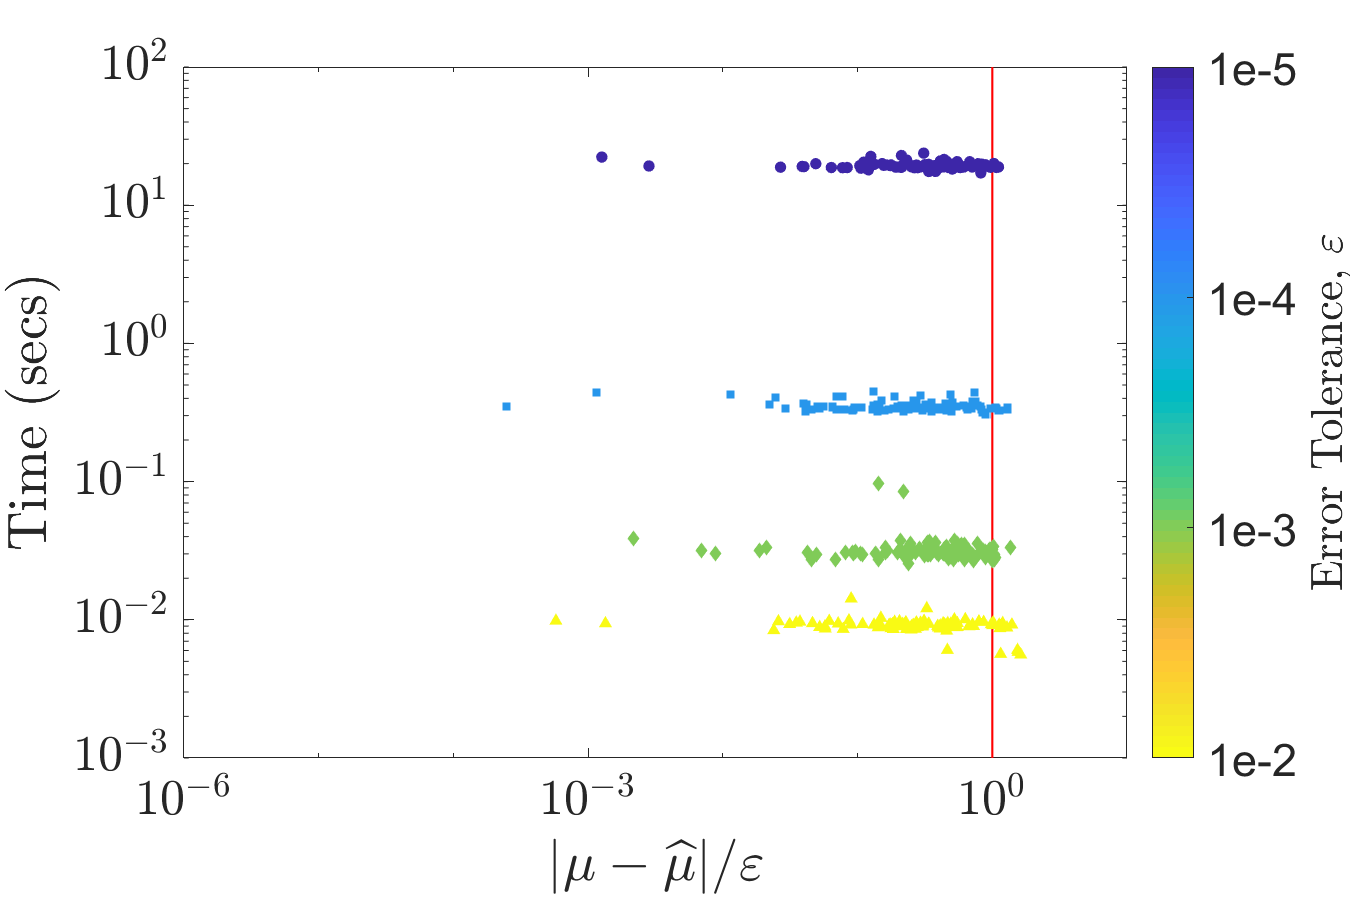
\includegraphics[height=4cm]{MVN_guaranteed_time_Matern_d2_2018-Aug-31}
\end{subfigure}
\centering
\begin{subfigure}[b]{0.49\textwidth}
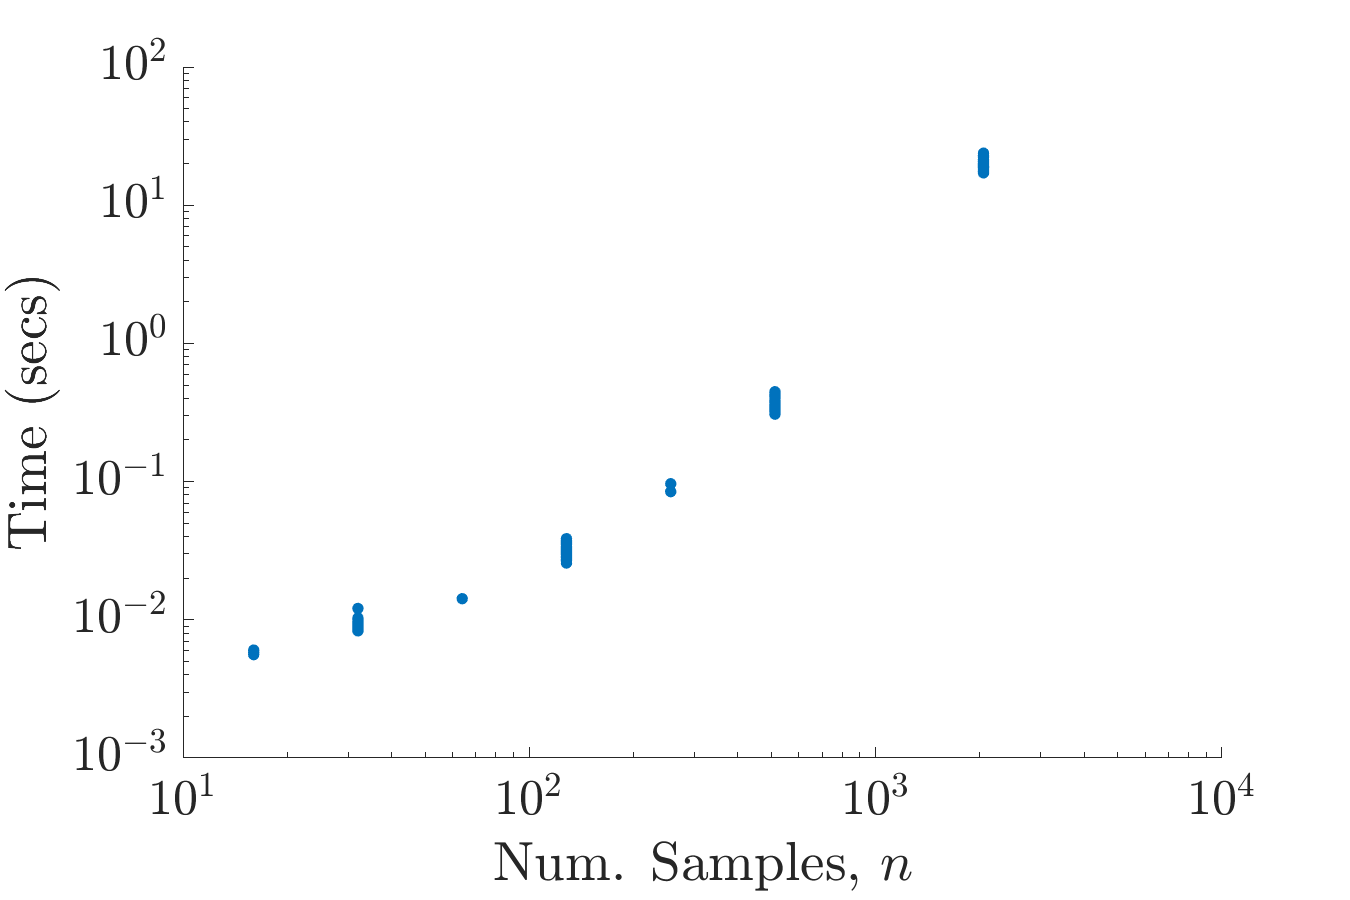
\includegraphics[height=4cm]{MVN_rapid_n_vs_time_Matern_d2_2018-Aug-31}
\end{subfigure}
%\caption{  }
\label{fig:MVN_Metern_d2b2}
\end{figure}
\alert{Problem}: Computation time (in seconds) increases rapidly, so it's not practical to use more than 4000 points in the cubature.
\end{frame}
















\section{Faster}



\subsection{Fast transform kernel}



\begin{frame}
\frametitle{Fast transform kernel}
\vspace{-5ex}
Choose the kernel $C_{\vtheta}$ and $\{\vx_i\}_{i=1}^n$, so the Gram matrix $\mC =  \left( C_{\vtheta} (\vx_i,\vx_j) \right)_{i,j=1}^n$ has the special properties:
\vspace{-2ex}
\begin{align*}
\mC =& \left( C_{\vtheta} (\vx_i,\vx_j) \right)_{i,j=1}^n 
= (\vC_1,...,\vC_n)
=  \frac 1n \mV \mLambda \mV^H 
\\
\mV :=& (\vv_1,...,\vv_n)^T = (\vV_1,...,\vV_n), \quad
\alert{\vV_1 = \vv_1 = \vone}, 
\\ 
\mLambda =& \diag (\vlambda), \quad \vlambda = (\lambda_1,...,\lambda_n)
\end{align*}
Then
\pause 
\vspace{-4ex}
\begin{align*}
\mV^H \vC_1 = \mV^H \left( \frac 1n \mV \mLambda \vv_1^* \right) =
 \mLambda \vone =
\begin{pmatrix}
\lambda_1, \hdots, \lambda_n
\end{pmatrix}^T = \vlambda
\end{align*}
\vspace{-1ex}
$C_{\vtheta}$ is a fast transform kernel, if the transform 
{\redroundmathbox{ { \text{$\hat{\vz} = \mV^H \vz$ }  } } }
for arbitrary $z$, can be done in \alert{$\Order( n \, log\, n) $}. Using the fast transform,
\vspace{-1ex}
\begin{align*}
\va^T\mC^p\vb &= \frac 1n \va^T \mV \mLambda^p \mV^H \vb
= \frac 1n \widetilde{\va}^H\mLambda^p \widetilde{\vb}
= \frac 1n \sum_{i=1}^n \lambda_i^p \widetilde{a}_i^* \widetilde{b}_i, 
\end{align*}
The covariance kernel used in practice also may be normalized 
$
\int_{[0,1]^d} C(\vt,\vx) \, \D \vt = 1 \qquad \forall \vx \in [0,1]^d,
$
leading to $c_0 = 1$ and $\vc = \vone$.
\end{frame}











\iffalse
\begin{frame}
\frametitle{Fast transform kernel --- More detailed}
\vspace{-5ex}
Choose the kernel $C_{\vtheta}$ and $\{\vx_i\}_{i=1}^n$ so the Gram matrix $\mC =  \left( C_{\vtheta} (\vx_i,\vx_j) \right)_{i,j=1}^n$ has the special properties
\vspace{-2ex}
\[
\begin{array}{lcc}
\quad
\mC =  \frac 1n \mV \mLambda \mV^H =  \frac 1n \mV^* \mLambda \mV^T = \mC^T,
\quad \quad
\mC^{-1} = \frac 1n \mV \mLambda^{-1} \mV^H = \frac 1n \mV^* \mLambda \mV^T,
\\
\mV := (\vv_1,...,\vv_n)^T = (\vV_1,...,\vV_n), \quad
\vV_1 = \vv_1 := \vone, \quad \mLambda = \diag (\lambda_1,...,\lambda_n)
\\ \pause
\\
\quad \quad
\mC \vone = \lambda_1 \vone, \quad \mC^{-1} \vone= \frac{1}{\lambda_1} \vone,
\quad \quad
\sum_{j=1}^n C(\vx_i, \vx_j) = \lambda_1, \; \forall i = 1,...,n,
\\
\mV^H = n \mV^{-1}, \quad \quad
\mV^H  \mV  = n
=
\mV^T \mV^* , \quad \quad c_0 := 1 \quad  \vc := \vone
\\ \pause
\\
\text{If} \quad
\mC = (\vC_1,...,\vC_n), \text{then}
\\
\mV^T \vC_1 = \mV^T \left( \frac 1n \mV^* \mLambda \vv_1 \right) =
\underbrace{\left( \frac 1n \mV^T  \mV^* \right) }_{I} \mLambda \vv_1  =  \mLambda \vone =
\begin{pmatrix}
\lambda_1 \\ \vdots \\ \lambda_n
\end{pmatrix}
\\
\text{A fast trasnform kernel $C_{\vtheta}$ is for which the transform }
{
\redroundmathbox{
{
\text{$\hat{\vz} = \mV^T \vz$ }
 } } }
\\
\text{can be done in $\Order( n \, log\, n) $}
\end{array}
\]
\end{frame}
\fi






\subsection{Shape param $\vthetaMLE$}


\frame{
\frametitle{Faster parameters estimation}
\vspace{-3ex}
MLE and GCV estimates of $\vtheta$ made faster by
using the properties of the fast transform kernel:
\vspace{-1ex}
\begin{align*}
\vthetaMLE &= 
\argmin_{\theta} \left[ \log\left(  \sum_{\alert{i=2}}^{n} \frac{|\hat{y}_i|^2}{\lambda_i} \right) + \frac{1}{n}\sum_{i=1}^{n} \log( \lambda_i ) \right],
\\
\vtheta_{\GCV} 
&= \argmin_{\vtheta} \left[ \log \left ( \sum_{\alert{i=2}}^n \frac{\abs{\widetilde{y}_i}^2}{\lambda_i^2} 
\right) -2\log\left( \sum_{i=1}^n \frac{1}{\lambda_i} \right)
\right], 
\end{align*}
\vspace{-3ex}
Also,
\begin{align*}
m_\MLE &= m_\GCV= \frac{1}{n} \sum_{i=1}^n y_i
, \quad
s^2_\MLE = \frac 1n \sum_{i=2}^n \frac{\abs{\hat{\vy}_i}^2}{\lambda_i}, 
\quad
s^2_{\GCV}  =  \frac 1{n} \sum_{i=2}^n \frac{\abs{\widetilde{y}_i}^2}{\lambda_i^2}  \left [ \sum_{i=1}^n \frac{1}{\lambda_i} \right]^{-1}
\\
\widehat{\sigma}^2_{\full}
&=
\frac{1}{n(n-1)} \sum_{i=2}^n \frac{\abs{\widetilde{y}_i}^2}{\lambda_i} \,  \left(\frac{\lambda_1}{n}  - 1  \right), \quad \text{where}
\end{align*}
\vspace{-3ex}
\begin{align*}
\hat{\vy} &= (\hat{y}_i)_{i=1}^{n} = \mV^T \vy ,
&   \vlambda &= ( \lambda_i )_{i=1}^{n} = \mV^T  \vC_1, \quad \text{where} \; \vC_1 =  \big( C(\vx_i, \vx_1) \big)_{i=1}^{n}
\end{align*}
\alert{$\Order(n \log n)$ operations to compute $\hat{\vy}$ and $\hat{\vlambda}$, So the $\vthetaMLE$}
}













\subsection{Error Bound}
\frame{
\frametitle{Computing the error bound $\err$ and $\hmu$ faster }
\vspace{-5ex}
Using the properties of the \alert{fast transform kernel}, the error bound \alert{$\errn$} can be computed faster
\vspace{-3ex} %\redroundmathbox
\begin{align*}
\;
\err_{\MLE} = 
\frac{2.58}{n} &\left\{ \sum_{i=2}^{n} \frac{\abs{\hy_i}^2}{\lambda_i}  
\left( 1 - \frac{n}{\lambda_1} \right)\right\}^{1/2}
\\
\err_{\full}
=
t_{n_j-1,0.995} &
\left\{\frac{1}{n(n-1)} \sum_{i=2}^n \frac{\abs{\widetilde{y}_i}^2}{\lambda_i} \, \left(\frac{\lambda_1}{n}  - 1  \right)\right\}^{1/2},
\\
\err_{\GCV}  =
\frac{2.58}{n} &
\left\{\sum_{i=2}^n \frac{\abs{\widetilde{y}_i}^2}{\lambda_i^2}  \left [ \frac 1n \sum_{i=1}^n \frac{1}{\lambda_i} \right]^{-1}  \times
\left( 1 -  \frac{n}{\lambda_1} \right)  
\right\}^{1/2}
\end{align*}
similarly, \alert{$\hmu$} can be computed faster
\vspace{-2ex}
\begin{align*}
&
\hmu_\MLE = \hmu_{\full} = \hmu_\GCV = \bm{w}^T \bm{y} =
\redroundmathbox{
\displaystyle{ \sum_{i=1}^n
\frac{{y}_i}{n} 
} }
\end{align*}
\vspace{-2ex}
where
\begin{align*}
\hvy = \mV^T \vy ,
\quad   \vlambda =  \mV^T \vC_1, \; \text{where} \; \vC_1 = \left( C(\vx_i, \vx_1) \right)_{i=1}^{n}
\end{align*}
\alert{$\Order(n \log n )$ operations to compute the $\err$}.
\alert{$\Order(n )$ operations to compute the $\hmu$}
}





\iffalse

\subsection{Algorithm - Bayesian Cubature}
\frame{
\frametitle{Automatic Bayesian Cubature}
\begin{algorithm}[H]
  \caption{Automatic Bayesian Cubature}\label{algorithm}
  \begin{algorithmic}[1]
    \Procedure{BayesCubature}{$f,\text{err}_{tol}$} \Comment{Integrate within the error threshold}
      \State $n \gets 2^8$
      \Do
        \State Generate Lattice points$(\vx_i)_{i=0}^{n-1}$
        \State Sample $(f(\vx_i))_{i=0}^{n-1}$
        \State Estimate optimal params $\vthetaMLE_n$
        \State Compute $\mathsf{C}_{\vthetaMLE, n}$
        \State Compute $\text{err}_{n}$
        \State $n\gets 2 \times n$
      \doWhile{$\text{err}_{n} > \text{err}_{tol}$}   \Comment{Iterate till error tolerance is met}
      \State Compute weights $(w_i)_{i=0}^{n-1}$
      \State Compute $\hmu_n$
      \State \textbf{return} $\hmu_n$ \Comment{Integral estimate $\hmu_n$}
    \EndProcedure
  \end{algorithmic}
\end{algorithm}
}

\fi







\iffalse
\begin{align*}
\text{Baker} & : & \tf(\vt)
= f\left(1-2|\vt-\frac{1}{2}| \right)
\\
\text{C0} & : & \tf(\vt)
= f\left(3\vt^2 - 2\vt^3\right)\prod_{j=1}^d(6t_j(1-t_j))
\\
\text{C1} & : & \tf(\vt)
= f\left(\vt^3(10-15\vt+6\vt^2)\right)\prod_{j=1}^d(30t_j^2(1-t_j)^2)
\\
\text{Sidi's C1} & : & \tf(\vt)
= f\left( \left( t_j- \frac{\sin(2\pi t_j)}{2\pi} \right)_{j=1}^d \right)\prod_{j=1}^d(1-\cos(2\pi t_j))
\end{align*}

%varies in terms of computational complexity and accuracy, choose based on the smoothness of the integrand.

\begin{enumerate}
\item Baker : Baker's transform or tent map in each coordinate. It preserves only continuity but it is easier to compute.
\item C0 : polynomial transformation only preserving continuity.
\item C1 : polynomial transformation preserving the first derivative.
\item C1sin : Sidi's transform with Sine, preserving the first derivative. This is in general a better option than 'C1'.
\end{enumerate}
\fi

































\section{Computational}


\subsection{Special covariance kernel }

\begin{frame}
\frametitle{Special shift invariant covariance kernel}
\vspace*{-8ex}
\begin{align*}
\redroundmathbox{
\displaystyle{
C_{\vtheta}(\vx, \vt) = \prod_{l=1}^d
1 - \theta_l^r  \frac{(2 \pi \sqrt{-1})^{r}}{r!} B_{r}( |{x_l-t_l}| ), \quad \vtheta \in (0,1]^d, \quad r \in 2\mathbb{N}}
}
\end{align*}
\vspace*{-0ex} 
\pause
where $B_r$ is Bernoulli polynomial of \alert{order $r$} \smallcite{OlvEtal10a}.
We call $C_{\vtheta}$, Fourier kernel. Also this kernel has:
\vspace*{-0ex}
\begin{align*}
\alert{c_0} &= \int_{[0,1]^2} C_{\vtheta} (\vx,\vt) \dvx \dvt = \alert{1}, 
\qquad
\alert{\vc} = \left( \int_{[0,1] } C_{\vtheta} (\vx_i,\vt) \dvt \right)_{i=1}^n = \alert{\vone}.
\\
\mV &= \Bigl ( \me^{2 \pi n \sqrt{-1} \phi(i-1)\phi(j-1)} \Bigr)_{i = 1}^n
\end{align*}

\end{frame}






\frame{
\frametitle{Fourier kernel}
\vspace{-5ex}
\begin{figure}[htp]
    \centering
    \begin{subfigure}[b]{0.40\textwidth}
    \includegraphics[width=\textwidth]{"fourier_kernel r_2 shape_10by100"}
    \end{subfigure}
    \centering
    \begin{subfigure}[b]{0.40\textwidth}
    \includegraphics[width=\textwidth]{"fourier_kernel r_2 shape_90by100"}
    \end{subfigure}
    \centering
    \begin{subfigure}[b]{0.40\textwidth}
    \includegraphics[width=\textwidth]{"fourier_kernel r_4 shape_10by100"}
    \end{subfigure}
    \centering
    \begin{subfigure}[b]{0.40\textwidth}
    \includegraphics[width=\textwidth]{"fourier_kernel r_4 shape_90by100"}
    \end{subfigure}
\end{figure}
}














\subsection{Rank-1 Lattice points}
\frame{ \frametitle{Rank-1 Lattice rules : low discrepancy point set }
\vspace{-5ex}
\only<1>{
Given the \alert{``generating vector'' $\vh$}, the construction of \alert{n} - Rank-1 lattice points \smallcite{DicPil10a} is given by
%\label{eqn:lattice_defn}
\begin{align}
\mathsf{L}_{n,\bm{h}} := \lbrace \vx_i :=  \bm{h} \phi(i-1)\; \textbf{mod} \; 1 ;\ \; i=1,\hdots,n
\rbrace
\end{align}
where $\bm{h}$ is a \emph{generalized Mahler integer} ($\infty$ digit expression) \smallcite{HicNie03a} also called \alert{generating vector}.
$\phi(i)$ is the Van der Corput sequence in base 2.
%Let us look at the construction of rank-1 lattice rules.
%Given a number of points \alert{$n$} and a \alert{``generating vecto'' $z$},
Then the Lattice rule approximation is
\[
\frac{1}{n} \sum_{k=1}^{n} f\left( \modop{ \frac{k \vh}{n} + \vDelta }_1 \right)
\]
where \alert{ $\modop{.}_1$} the fractional part, i.e, \emph{modulo 1} operator and $\vDelta$ a random shift.

\emph{Extensible integration lattices} : The number of points in the node set can be increased while retaining the existing points.\smallcite{HicNie03a}
}

%\only<2>{
%\centering\redroundmathbox{\text{
%Shift invariant kernel + Lattice points = `\emph{Symmetric circulant %kernel}' matrix
%}}
%}

}




\frame{
\frametitle{Rank-1 Lattice points in $d=2$}
\vspace{-5ex}
\begin{figure}[htp]
    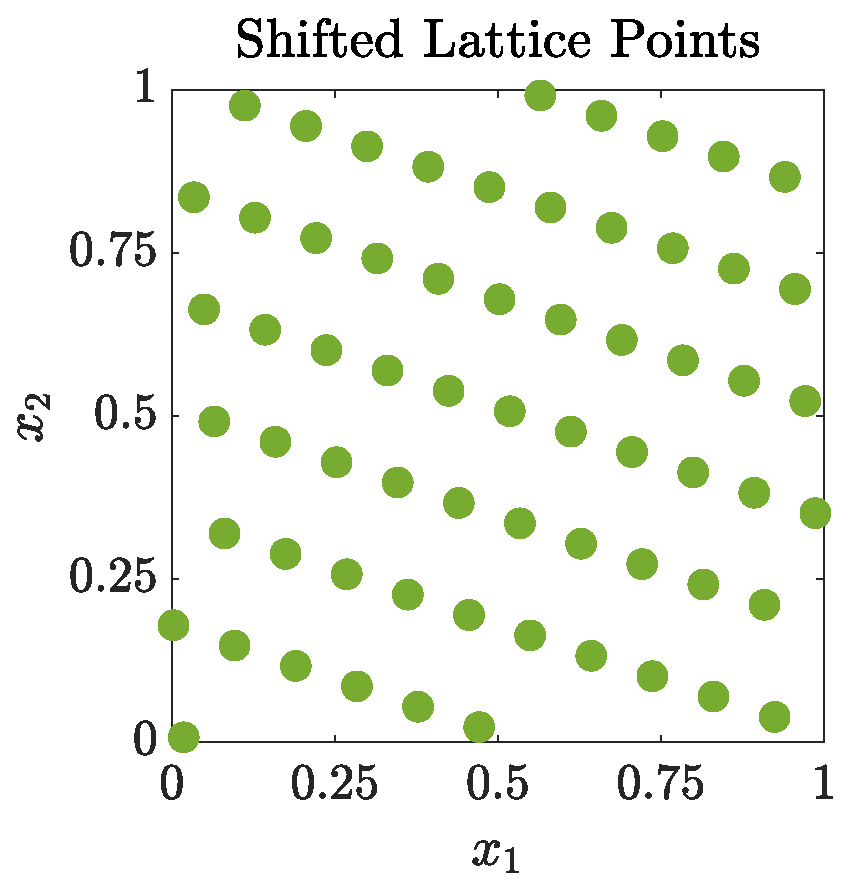
\includegraphics[height=5cm]{figures/ShiftedLatticePoints}
\end{figure}

\centering\redroundmathbox{\text{
Shift invariant kernel + Lattice points = `\emph{Symmetric circulant kernel}' matrix
}}
}








\frame{
\frametitle{ The shift invariant kernel with rank-1 Lattice points}
\vspace{-7ex}
\begin{minipage}{\textwidth}
\linespread{2}
\begin{itemize}
\item Satisfies all the requirements to be a \alert{fast transform kernel}
\item Fast transform = fast Fourier transform
\item Complexity of fast Fourier transform is \alert{$\Order(n \log n)$}
\item No need to form the kernel matrix $\mC$ explicitly, so $\Order(n^2)$ memory not required
\item There are \alert{no} matrix inversions, \alert{no} matrix multiplications
\item Factorization of matrix $\mC$ does not need any computations.
\\
 where $\mV$ is just the Fourier coefficient matrix: $\mV = \Bigl ( \me^{2 \pi n \sqrt{-1} (i-1)(j-1)} \Bigr)_{i = 1}^n $
\end{itemize}
\end{minipage}
}










\subsection{Iterative DFT}
\frame{ \frametitle{Iterative DFT}
\vspace{-7ex}
We can avoid recomputing the whole Fourier transform for function values $vy = \left(y_i = f(\vx_i) \right)_{i=1}^n$ in every iteration.
Discrete Fourier transform is defined as
\begin{align*}
\mathcal{DFT} \{y \} := \hat{y} = \left( \sum_{j=1}^{n} y_j
e^{-\frac{2\pi \sqrt{-1}}{n} (j-1) (i-1) }
\right)_{i=1}^{n}
, \quad
\hat{y}_i &=  \sum_{j=1}^{n} y_j
e^{- \frac{2\pi \sqrt{-1}}{n} (j-1) (i-1) }
\end{align*}
\pause
Rearrange sum into even indexed $j=2l$ and odd indexed $j=2 l + 1$.
\begin{align*}
\hat{y}_i &=
\underbrace{
\sum_{l=1}^{n/2} y_{2l}
e^{- \frac{2\pi \sqrt{-1}}{n/2} (l-1)( i-1) }
}_{\text{DFT of even-indexed part of}\; y_i}
+
e^{- \frac{2\pi \sqrt{-1}}{n} (i-1) }
\underbrace{
\sum_{l=1}^{n/2} y_{2l+1}
e^{- \frac{2\pi \sqrt{-1}}{n/2} (l-1)( i-1) }
}_{\text{DFT of odd-indexed part of}\; y_i}
\end{align*}
we use this concept along with \emph{extensible point set}, to avoid recomputing the DFT of $\vy$ in every iteration.
}











\subsection{Cancellation error in $\err$}
\frame{ \frametitle{Cancellation error in $\err$}
\vspace{-7.5ex}
\begin{align*}
\errn =
2.58\sqrt{\left( 1 - \frac{n}{\lambda_1} \right) \,
\frac {1}{n^2} \sum_{i=2}^{n} \frac{\abs{\hy_i}^2}{\lambda_i}  }
,
\quad \text{term $\alert{ 1 - \frac{n}{\lambda_1} }$ causes cancellation error}
\end{align*}
\pause
\vspace{-2ex}
\begin{align*}
\text{Let}\; \tC(\vx, \vt) = C(\vx, \vt) - 1,
\quad
\text{then} \; \tmC = \mC - \vone \vone^T, \quad \text{and} \; \tmC = \mV \tmLambda \mV^H
\end{align*}
where
\vspace{-3ex}
\begin{align*}
\tmLambda &= \diag(\tlambda_1, ..., \tlambda_n), \; \text{to compute} \;
\redroundmathbox{ \displaystyle{
 (\tlambda_i)_{i=1}^n = \mV^T \tvC_1
} }
\\
\tlambda_1 &=  \lambda_1 - n,
\quad
\tlambda_j = \lambda_j, \; \forall \; j=2,...,n
\end{align*}
\vspace{-3ex} \pause
\begin{align*}
\text{vector} \; \tvC_1 = \tvC_1^{(d)} &\; \text{computed iteratively }
\\
\tvC_1^{(1)} &= \theta \; \bigl( B(x_{i1} - x_{11}) \bigr)_{i=1}^n ,
\quad \;
\vC_1^{(1)} = \vone + \tvC_1^{(1)},
\\
\forall 1 < k \leq d, \quad \tvC_1^{(k)} &=  \theta  \vC_1^{(k-1)} \alert{\circ} \bigl( B(x_{ik} - x_{1k}) \bigr)_{i=1}^n  + \tvC_{k-1}, \quad \vC_1^{(k)} = \vone + \tvC_1^{(k)}
\\
&\text{where $\alert{\circ}$ is elementwise multiplication. MATLAB=.*}
\end{align*}
Using this to avoid cancellation error
\vspace{-3ex}
\[
1 - \frac{n }{\lambda_1}
=  1 - \frac{n }{n+ \tlambda_1}
=
\redroundmathbox{ \displaystyle{
\frac{\tlambda_1 }{n+ \tlambda_1}
} }
\]
}










\iffalse
\subsection{Asserting Gaussian process assumption}

\frame{
\frametitle{Asserting Gaussian process assumption}
\vspace{-5ex}
How can we check if $m, s, \vtheta$ and $\mC$ are chosen well, So $\vf$ is a draw from the Gaussian process?
\vspace{-2ex}
\begin{align*}
\vf = \left( f(\vx_i) \right)_{i=1}^n
\sim \mathcal{N} \left( m\vone, s^2 \mC \right), &
\quad \text{where}\quad \mC = \frac 1n \mV \mLambda \mV^H, \quad \mV^H \mV = n 
\\
\text{Let} \quad \vf' = \frac{1}{\sqrt{n}} \mLambda^{-\frac 12} \mV^H \vf, & 
\end{align*}
\vspace{-6ex}
\begin{align*}
\text{Then}, \quad
\mathbb{E}\left[ \vf' \right]
 &=
\frac{1}{\sqrt{n}} \mLambda^{-\frac 12} \mV^H \mathbb{E}[\vf] 
 = m \sqrt{\frac{n}{\lambda_1}} \left( 
\begin{array}{c}
1 \\ 0 \\ \vdots \\ 0
\end{array}
\right),
\\
COV \left[ \vf'  \right]
&=
\frac{1}{n} \mathbb{E}\left[  
\mLambda^{-\frac 12} \mV^H (\vf - m \vone)
(\vf - m \vone)^T \mV \mLambda^{-\frac 12}
\right]
\\
&=
\frac{1}{n} \mLambda^{-\frac 12} \mV^H 
\frac 1n \mV \mLambda \mV^H \mV \mLambda^{-\frac 12}
 = \quad \mathsf{I}
\\
\text{Thus, the distribution of,} \quad
\vf' &\sim \mathcal{N} \left( 
m' \bm{e}_1,
\mathsf{I}
\right), \text{Where $m' = m \sqrt{\frac{n}{\lambda_1}} $.}
\end{align*}
If we can verify the sample distribution of $\vf'$ is $\mathcal{N}\left( m' \bm{e}_1, \mathsf{1} \right)$, It could validate our assumption.


}






\begin{frame}
\frametitle{Normal plots}
\vspace{-5ex}
\begin{figure}[htp]
\captionsetup[subfigure]{labelformat=empty}
\centering
\begin{subfigure}[b]{0.49\textwidth}
\includegraphics[height=4cm]{"arbMean/Keister/C1sin/Keister Normplot d_2 bernoulli_2 Period_C1sin n_32768"}
\end{subfigure}
\centering
\begin{subfigure}[b]{0.49\textwidth}
\includegraphics[height=4cm]{"arbMean/MVN/C1sin/MVN Normplot d_2 bernoulli_2 Period_C1sin n_32768"}
\end{subfigure}
\caption{ Left : Keister, Right : MVN normplots}
%\label{fig:MVN_Metern_d2b2}
\end{figure}
\vspace{-3ex}
shows the $\vf'$ is approximately Gaussian distributed.
\vspace{-3ex}
\begin{itemize}
\item
Keister example is with C1sin transform and Bernoulli order $r=2$ and dimension $d=2$.
\item
MVN example is also with C1sin transform and Bernoulli order $r=2$ and dimension $d=2$.
\end{itemize}
\end{frame}

\fi



\subsection{Periodization transforms}
\frame{\frametitle{Periodization transforms}
\vspace*{-8ex}
\setlength{\abovedisplayshortskip}{-1pt}
\setlength{\belowdisplayshortskip}{0pt}
\[
\begin{array}{rcll}
\text{Baker's} & : \tilde{f}(\vt) &
= f\left( \left(1-2 \abs{t_j-\frac{1}{2}} \right)_{j=1}^d \right)
\\
\text{C0} & : \tilde{f}(\vt) &
= f\left( \bar{g}_0(\vt) \right)\prod_{j=1}^d g'_0(t_j), \quad
g_0(t) = 3 t^2 - 2 t^3, \quad  g'_0(t) = 6t(1-t))
\\
\text{C1} & :  \tilde{f}(\vt) &
= f\left( \bar{g}_1(\vt)\right)\prod_{j=1}^d g'_1(t_j),
\\
& &
g_1(t) = t^3(10-15t+6t^2), \quad  g'_1(t) = 30t^2(1-t)^2
\\
\text{Sidi's C1} & :  \tilde{f}(\vt) &
= f\left( \bar{\psi}_2(\vt) \right) \prod_{j=1}^d \psi'_2(t_j)
\\
& & \psi_2(t) =
\left(t - \frac{1}{2\pi} \sin(2\pi t) \right)
, \quad
\psi'_2(t) = \left(1 - \cos(2 \pi t)  \right)
\\
\text{Sidi's C2} & :  \tilde{f}(\vt) &
= f\left( \bar{\psi}_3(\vt) \right) \prod_{j=1}^d \psi'_3(t_j),
\quad
\psi_3(t) =
\frac{1}{16} \left(8-9\cos(\pi t)+ \cos(3\pi t) \right),
\\
& &
\psi'_3(t) =
\frac{1}{16} \left(9 \sin(\pi t) \pi - \sin(3 \pi t) 3 \pi \right)
\end{array}
\]
%please note that, we use the shortened vector notation for $g(.) : \mathbb{R} \to \mathbb{R}$
% \begin{align*} \bar{g}(\vt) = \left( g(t_j) \right)_{j=1}^d \end{align*}
%These transforms vary in terms of computational complexity and accuracy, shall be chosen on a need basis.
}








\section{Experiments}


\iffalse
\subsection{Test functions}
\frame{
\frametitle{Test functions for Numerical integration:}
\vspace{-8ex}
\begin{tabular}{m{8.5cm}m{3cm}}
{Multivariate Normal (MVN)} \vspace{-2ex}
\begin{gather*}
\mu = \int_{[\va,\vb]} \frac{\exp\bigl(- \frac 12 \vt^T \mSigma^{-1} \vt \bigr)}{\sqrt{(2 \pi)^d \det(\mSigma)}} \, \dif \vt \
\overset{\text{\smallocite{Gen93}}}{=} \
\int_{[0,1]^{d-1}} f(\vx) \, \dif \vx
\end{gather*} &
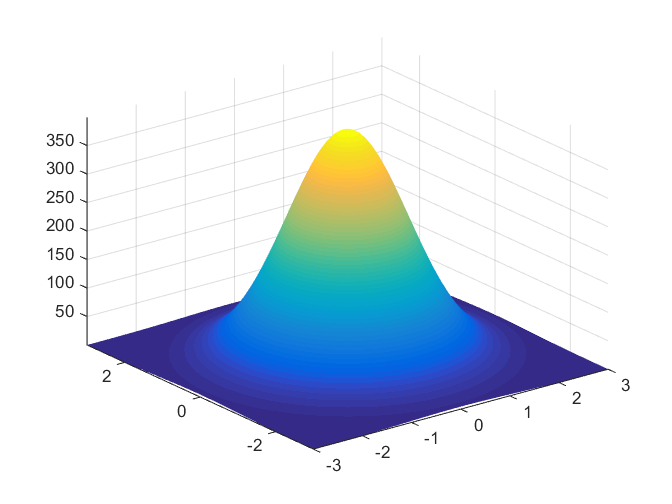
\includegraphics[width=3cm,angle=0]{Plotting_gaussian.png}
\end{tabular}
\begin{align*}
\text{Keister} &:& \mu &= \int_{\mathbb{R}^d} \cos(\lVert \boldsymbol{x} \rVert)
\exp(-\lVert \boldsymbol{x} \rVert^2) \, \mathrm{d} \boldsymbol{x},
& d = 1, 2, \ldots. & &
\\
\text{Exp(Cos)} &:& \mu &= \int_{(0,1]^d} \exp(\cos (\vx ) ) \mathrm{d} \boldsymbol{x},
& d = 1, 2, \ldots. & &
\end{align*}

}
\fi


















































\iffalse


\subsection{computation time with shift invariant kernel}
\begin{frame}
\frametitle{Computation time with Fourier kernel}
\vspace{-1ex}
\begin{figure}[htp]
\captionsetup[subfigure]{labelformat=empty}
\centering
%\begin{subfigure}[b]{0.99\textwidth}
\includegraphics[height=5cm]{zeroMean/MVN/C1sin/"MVN computeTime d_2 bernoulli_2 Period_C1sin"}
%\end{subfigure}
\caption{ MVN : d=2 r=2, C1sin }
%\label{fig:MVN_Metern_d2b2}
\end{figure}
\vspace{-3ex}
Computation time increases linearly, so we can use more than 4000 points in the Cubature, upto $2^{23}$ points with 16GB RAM computer.
\end{frame}


\fi








\subsection{Automatic cubature}





\iffalse
\begin{frame}
\frametitle{Error bound vs actual error - Automatic cubature}
\vspace{-5ex}
\begin{figure}[htp]
\captionsetup[subfigure]{labelformat=empty}
\centering
\begin{subfigure}[b]{0.49\textwidth}
\includegraphics[height=4cm]{"AsianArithmeticMeanOption error_vs_errbd"}
\end{subfigure}
\centering
\begin{subfigure}[b]{0.49\textwidth}
\includegraphics[height=4cm]{"MVN error_vs_errbd"}
\end{subfigure}
\caption{ Left : OptionPricing, Right : MVN with various error bounds}
%\label{fig:MVN_Metern_d2b2}
\end{figure}
\vspace{-3ex}
shows the Automatic Bayesian cubature algorithm meets the error bound $\errn$.
\vspace{-3ex}
\begin{itemize}
\item
Option pricing example is only with Baker transform and Bernoulli order $r=2,4$.
\item
MVN example uses Baker, C1sin and C2sin transforms, Bernoulli order $r=2,4$ and dimension $d=2,3$.
\end{itemize}
\end{frame}
\fi


\iffalse
\begin{frame}
\frametitle{Error vs Time - Automatic cubature}
\vspace{-5ex}
\begin{figure}[htp]
\captionsetup[subfigure]{labelformat=empty}
\centering
\begin{subfigure}[b]{0.49\textwidth}
\includegraphics[height=4cm]{"AsianArithmeticMeanOption errorVtime"}
\end{subfigure}
\centering
\begin{subfigure}[b]{0.49\textwidth}
\includegraphics[height=4cm]{"MVN errorVtime 1"}
\end{subfigure}
\caption{ Left : OptionPricing $\errtol=10^{-2}$, Right : MVN $\errtol=10^{-4}$}
%\label{fig:MVN_Metern_d2b2}
\end{figure}
\vspace{-3ex}
shows the Automatic Bayesian cubature algorithms meets the specified $\errtol$ in a less than few seconds.
\vspace{-3ex}
\begin{itemize}
\item
Option pricing example is only with Baker transform and Bernoulli order $r=2,4$.
\item
MVN example uses Baker, C1sin and C2sin transforms, Bernoulli order $r=2,4$ and dimension $d=2,3$.
\end{itemize}
\end{frame}
\fi











\subsection{MVN}


\iffalse
\frame{
\frametitle{Multivariate normal probability with fixed mean $m=0$}
\vspace{-5ex}
\begin{figure}[htp]
    \centering
    \begin{subfigure}[b]{0.34\textwidth}
    \includegraphics[width=\textwidth]{zeroMean/MVN/C1sin/"MVN Error d_2 bernoulli_2 Period_C1sin"}
    \end{subfigure}
    \centering
    \begin{subfigure}[b]{0.34\textwidth}
    \includegraphics[width=\textwidth]{zeroMean/MVN/C1sin/"MVN Error d_3 bernoulli_2 Period_C1sin"}
    \end{subfigure}
    \centering
    \begin{subfigure}[b]{0.34\textwidth}
    \includegraphics[width=\textwidth]{zeroMean/MVN/C1sin/"MVN Error d_2 bernoulli_4 Period_C1sin"}
    \end{subfigure}
    \centering
    \begin{subfigure}[b]{0.34\textwidth}
    \includegraphics[width=\textwidth]{zeroMean/MVN/C1sin/"MVN Error d_3 bernoulli_4 Period_C1sin"}
    \end{subfigure}
\end{figure}
}
\fi


\frame{
\frametitle{Multivariate normal probability }
\vspace{-5ex}
\begin{figure}[htp]
    \centering
    \begin{subfigure}[b]{0.43\textwidth}
    \includegraphics[width=\textwidth]{"MVN_guaranteed_time_MLE_C2sin_d2_r2_2018-Sep-6"}
    \end{subfigure}
    \centering
    \begin{subfigure}[b]{0.43\textwidth}
    \includegraphics[width=\textwidth]{"MVN_guaranteed_time_GCV_C2sin_d2_r2_2018-Sep-6"}
    \end{subfigure}
    \centering
    \begin{subfigure}[b]{0.43\textwidth}
    \includegraphics[width=\textwidth]{"MVN_guaranteed_time_full_C2sin_d2_r2_2018-Sep-6"}
    \end{subfigure}
\caption{Multivariate normal probability example using 1) Empirical Bayes, 2) GCV, 3) Full Bayes stopping criterion}
\end{figure}
}


\subsection{Keister integral}


\frame{
\frametitle{Keister Integral with arb mean $m$}
\vspace{-5ex}
\begin{figure}[htp]
	\linespread{0.7}
    \centering
    \begin{subfigure}[b]{0.43\textwidth}
    \includegraphics[width=\textwidth]{"Keister_guaranteed_time_MLE_C1sin_d4_r2_2018-Sep-6"}
    \end{subfigure}
    \centering
    \begin{subfigure}[b]{0.43\textwidth}
    \includegraphics[width=\textwidth]{"Keister_guaranteed_time_GCV_C1sin_d4_r2_2018-Sep-6"}
    \end{subfigure}
    \centering
    \begin{subfigure}[b]{0.43\textwidth}
    \includegraphics[width=\textwidth]{"Keister_guaranteed_time_full_C1sin_d4_r2_2018-Sep-6"}
    \end{subfigure}
   \caption{Integrating Keister function using 1) Empirical Bayes, 2) GCV, 3) Full Bayes stopping criterion}
\end{figure}
}



\subsection{Option pricing}

\frame{
	\frametitle{Option pricing}
	\vspace{-5ex}
	\begin{figure}[htp]
		\linespread{0.7}
		\centering
		\begin{subfigure}[b]{0.43\textwidth}
			\includegraphics[width=\textwidth]{"optPrice_guaranteed_time_full_Baker_d12_r1_2018-Sep-6"}
		\end{subfigure}
		\centering
		\begin{subfigure}[b]{0.43\textwidth}
			\includegraphics[width=\textwidth]{"optPrice_guaranteed_time_GCV_Baker_d12_r1_2018-Sep-6"}
		\end{subfigure}
		\centering
		\begin{subfigure}[b]{0.43\textwidth}
			\includegraphics[width=\textwidth]{"optPrice_guaranteed_time_full_Baker_d12_r1_2018-Sep-6"}
		\end{subfigure}
		\caption{Option pricing using 1) Empirical Bayes, 2) GCV, 3) Full Bayes stopping criterion}
	\end{figure}
}


































l\section{Conclusion}
\frame{\frametitle{Summary}
\begin{minipage}{\textwidth}
\linespread{1.3}
\begin{itemize}
\item Developed a \emph{general technique} for a \alert{Fast transform kernel}
\item Developed a \alert{fast automatic Bayesian cubature} with \alert{$\Order(n\log n)$} complexity
\item Having the advantages of a kernel method and the low computation cost of Quasi Monte carlo
\item Scalable based on the complexity of the Integrand
\\ i.e, Kernel order and Lattice-points can be chosen to suit the smoothness of the integrand
\item Conditioning problem if the kernel $C$ is very smooth
\item Source code : \alert{\url{https://github.com/GailGithub/GAIL_Dev/tree/feature/BayesianCubature}}
\item More about Guaranteed Automatic Algorithms (GAIL): \alert{\url{http://gailgithub.github.io/GAIL_Dev/}}
%\item These slides will also be available at slideshare.net
\end{itemize}
\end{minipage}
}


\section{Future work}
\frame{\frametitle{Future work}
\begin{minipage}{\textwidth}
\linespread{1.6}
\begin{itemize}
\item Choosing the \alert{kernel order $r$} and \alert{periodization} transform automatically
\item \alert{Deterministic} interpretation of Bayesian cubature
\item Broaden the choice of numerical examples
\item Better handling of \alert{conditioning} problem and numerical  errors
\\
\item Sobol pointset and Fast Walsh Transform with smooth kernels ...
\end{itemize}
\end{minipage}
}


\frame{\frametitle{Future work : Sobol points and Fast walsh transform}

\begin{itemize}
\vspace{-3ex}
\item
Using the established generalized theory for a \textit{Fast transform kernel}, we could use other kernels with suitable point sets to achieve similar or better performance and accuracy. 
\item
One such point sets to consider in future is, \textit{Sobol points} and with appropriate choice of smooth kernel, should lead to \textit{Fast Walsh Transform}.
\end{itemize}
\vspace{-3ex}
%\begin{figure}[htp]
%    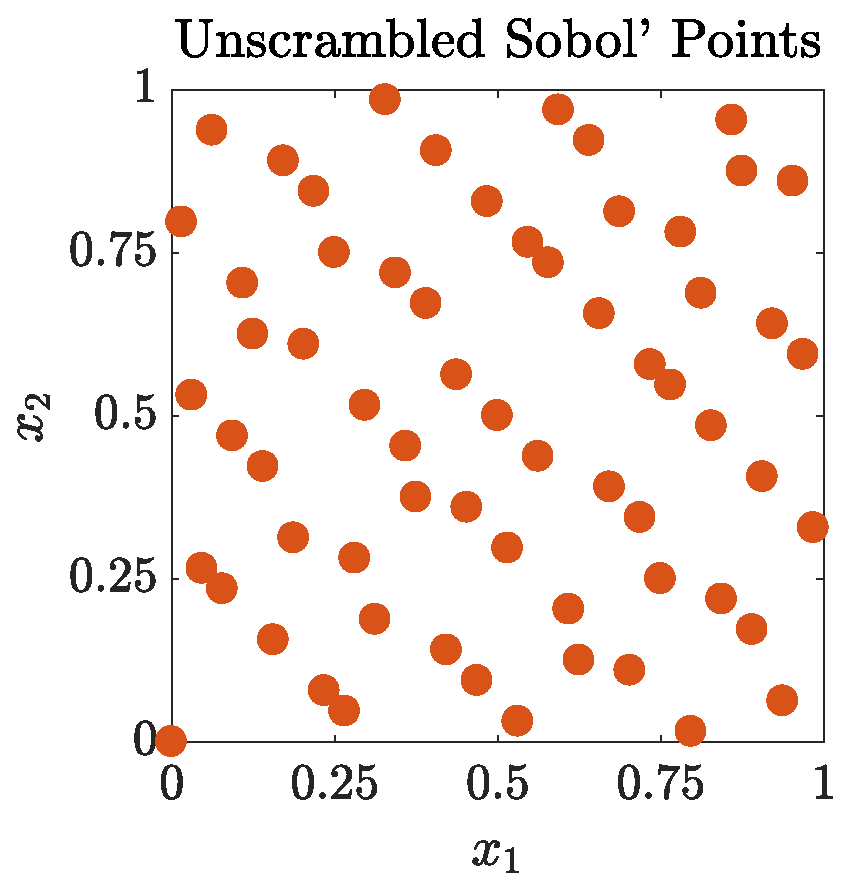
\includegraphics[height=5cm]{figures/USobolPoints}
%\end{figure}
\begin{figure}[htp]
    \centering
    \begin{subfigure}[b]{0.35\textwidth}
    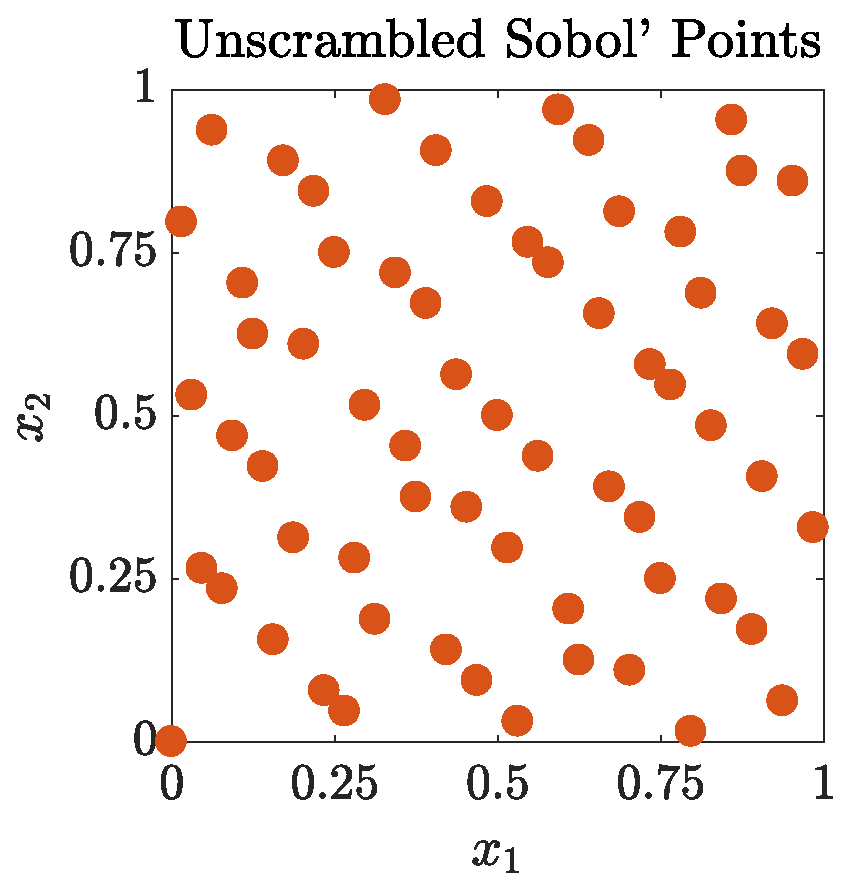
\includegraphics[width=\textwidth]{figures/USobolPoints}
    \end{subfigure}
    \centering
    \begin{subfigure}[b]{0.35\textwidth}
    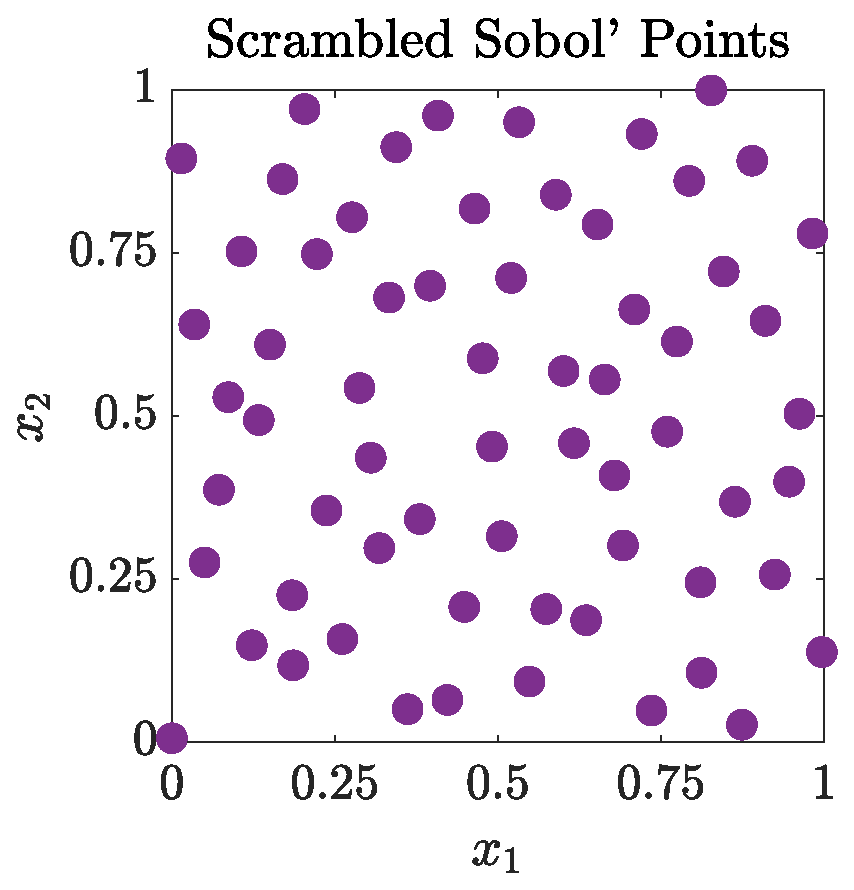
\includegraphics[width=\textwidth]{figures/SSobolPoints}
    \end{subfigure}
\end{figure}
}

\frame{\frametitle{Future work : More applications}
\vspace{-4ex}
\begin{itemize}
\item \alert{Control variates} : 
We would like to approximate a function of the form
$ (f - \beta_1 g_1 -, ... , - \beta_p g_p) $, then
\begin{align*}
f = \mathcal{N} \left( \beta_0 + \beta_1 g_1 + , ... , + \beta_p g_p, s^2 \mC  \right)
\end{align*}
\item \alert{Function approximation} : 
consider approximating a function of the form
\begin{align*}
\int_{[0,1]^d} \underbrace{ f(\vphi(\vt)) . \abs{\frac{\partial \vphi}{\partial \vt}} }_{g(\vt)} \dvt,&
\quad 
\text{where $\abs{\frac{\partial \vphi}{\partial \vt}}$ is Jacobian, then}&
\\
g(\vpsi(\vx)) = f( \underbrace{ \vphi(\vpsi(\vx) }_{\vx } ) .& \abs{\frac{\partial \vphi}{\partial \vt} }  (\vpsi(\vx)),
\quad
f(\vx) = g(\vpsi(\vx)) . \frac{1}{  \abs{\frac{\partial \vphi}{\partial \vt}}  (\vpsi(\vx)) }
\end{align*}
Finally, the function approximation is
\begin{align*}
\tilde{f}(\vx) &= \tilde{g}(\vpsi( \vx )) \\
&= \sum w_i C(.,.)
\end{align*}
\end{itemize}
}

\iffalse

\frame{
\frametitle{Low discrepancy points}
\vspace{-5ex}
\begin{figure}[htp]
    \centering
    \begin{subfigure}[b]{0.35\textwidth}
    \includegraphics[width=\textwidth]{figures/IIDPoints}
    \end{subfigure}
    \centering
    \begin{subfigure}[b]{0.35\textwidth}
    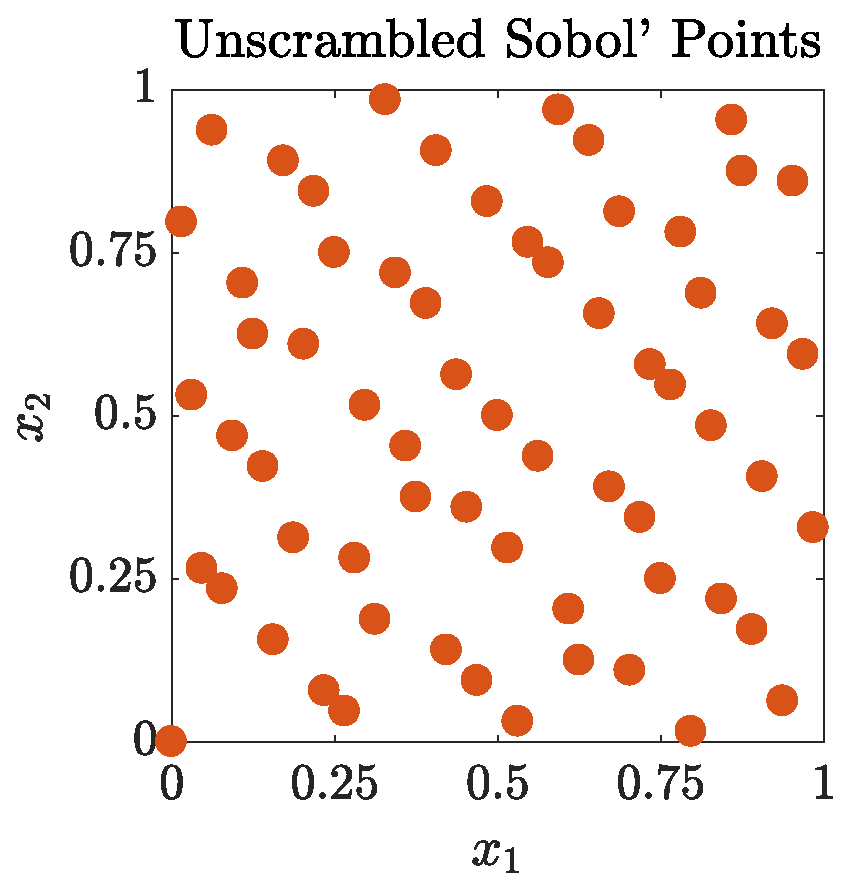
\includegraphics[width=\textwidth]{figures/USobolPoints}
    \end{subfigure}
    \centering
    \begin{subfigure}[b]{0.35\textwidth}
    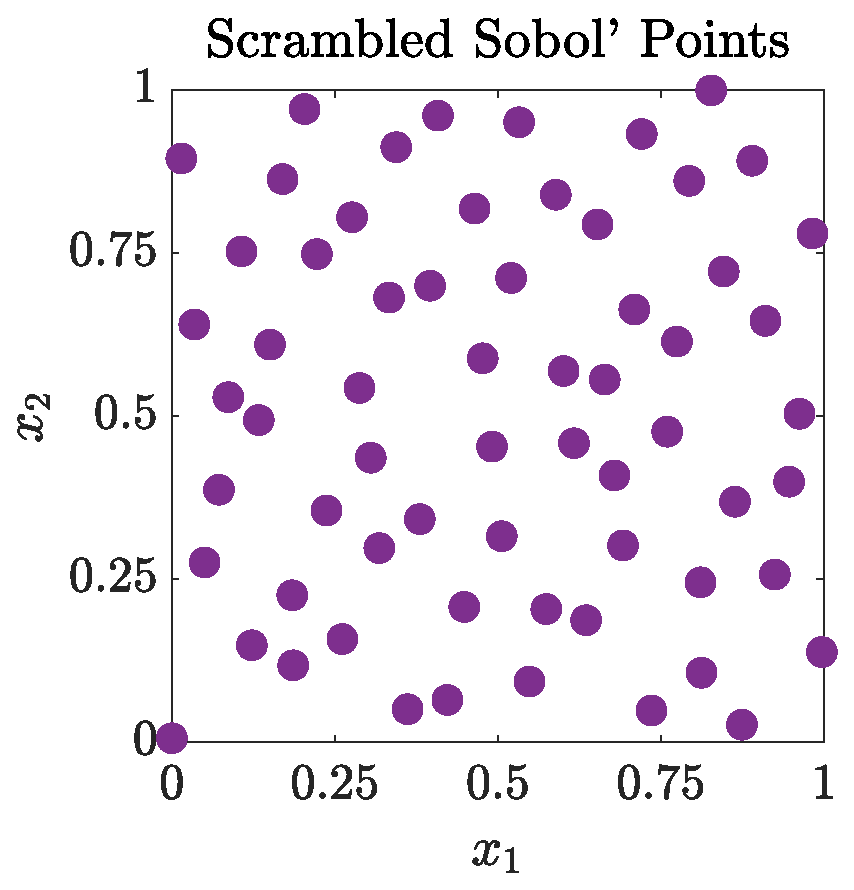
\includegraphics[width=\textwidth]{figures/SSobolPoints}
    \end{subfigure}
    \centering
    \begin{subfigure}[b]{0.35\textwidth}
    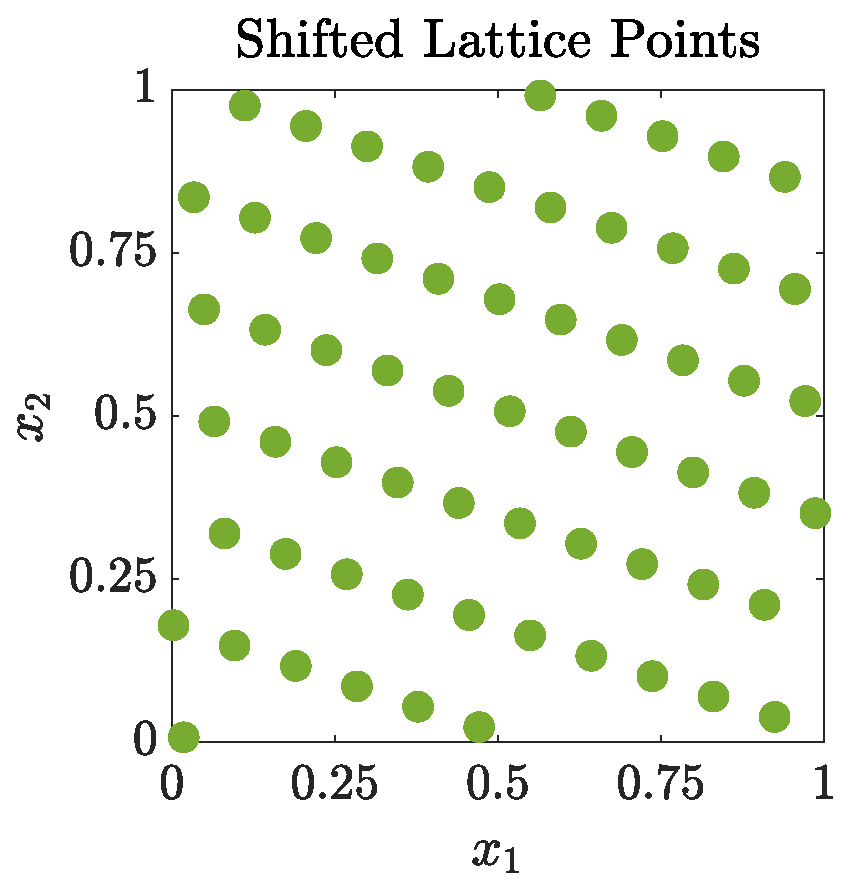
\includegraphics[width=\textwidth]{figures/ShiftedLatticePoints}
    \end{subfigure}
\end{figure}
}
\fi

%\thankyouframe

\begin{frame}[plain,c]
%\frametitle{A first slide}

\begin{center}
\Huge Thank you!
\end{center}

\end{frame}


\begin{frame}[allowframebreaks]\frametitle{References}
	\bibliography{FJH22,FJHown22}{}
	%\bibliography{../mybib}{}
\end{frame}

\end{document}
